\clearpage
% Set chapter counter to 2 and reset section counter
\setcounter{chapter}{2}
\setcounter{section}{0}

% Add the chapter to table of contents
\addcontentsline{toc}{chapter}{\numberline{2}Rethinking Democratization: Beyond Access to Preservation}

% Set up page style for this chapter (assuming fancyhdr is loaded in preamble)
\pagestyle{fancy}
\fancyhf{} % Clear all header and footer fields
\fancyhead[L]{\footnotesize\textit{Ars Post Faber: Digital Fabrication Democratization Through Embodied Knowledge Preservation}}
\fancyfoot[C]{\thepage} % Page number in footer center
\renewcommand{\headrulewidth}{0pt}
\renewcommand{\footrulewidth}{0pt}

% Custom chapter title to match abstract formatting
\noindent
{\Large\textbf{Chapter 2: Rethinking Democratization: Beyond Access to Preservation}}
\vspace{0.3cm}
\hrule
\vspace{0.8cm}
\label{ch:democratization}

% Set no paragraph indentation
\setlength{\parindent}{0pt}

The historical trajectory examined in Chapter 1 has showed how creative agency has been systematically redistributed from unified practice to contemporary digital workflows. This analysis raises the question: if digital fabrication technologies possess unprecedented capabilities for material manipulation and geometric exploration, why do they continue to perpetuate the same distributed agency frameworks that eliminated adaptive authority? The answer lies in how the "democratization" itself has been conceptualized within digital fabrication discourse.

\vspace{0.5cm}

Rather than addressing the organizational structures that fragment creative agency, contemporary digital fabrication has pursued democratization primarily through expanded access to scaled-down industrial tools. This chapter will examine how this access-centered approach, while achieving remarkable quantitative success, fails to address the deeper structural issues identified in the historical analysis. By tracing the evolution from access-based democratization toward preservation-centered approaches, this chapter will try to pursue a reconceptualization of what democratic making might mean in digital contexts.

\section{The Access Paradigm and Its Achievements}

This access-centered understanding of democratization has become the dominant paradigm within contemporary digital fabrication discourse. Neil Gershenfeld's\footnote{Neil Gershenfeld is a physicist at MIT who's the director of the Center for Bits and Atoms (CBA) and pioneered the global FabLab movement. His work focuses on the intersection of physical and digital systems, advocating for "personal fabrication" as a means to democratize access to manufacturing capabilities.} foundational vision for FabLabs\footnote{FabLabs (Fabrication Laboratories) are digital fabrication workshops that provide public access to tools for invention, prototyping and local production. Originally conceived at MIT's Center for Bits and Atoms, FabLabs follow a global charter emphasizing open access, education, and local innovation while connecting to a worldwide network of collaborative spaces.} promised "personal fabrication" enabling "almost anyone to make almost anything" \citep{gershenfeld2007}, positioning digital fabrication as the natural evolution of personal computing—bringing the same accessibility that desktop computers brought to information processing into the realm of physical manufacturing. This vision emphasized scaling down industrial production capabilities to individual users, making sophisticated fabrication tools available in community workshops and educational institutions.

\vspace{0.5cm}

Building on this foundation, the broader maker movement, as articulated by Mark Hatch, advocated for "radically democratizing access to the tools of innovation" \citep{hatch2013}, framing making as both a form of personal empowerment and economic opportunity. Hatch's manifesto positioned the maker movement as a response to mass production's alienation, promising that widespread access to fabrication tools would restore individual agency in production while fostering innovation and entrepreneurship at the grassroots level.

\vspace{0.5cm}

This approach has achieved remarkable quantitative success: from fewer than 50 FabLabs worldwide in 2009 to over 2,000 by 2023 (Fab Foundation, 2024), there's been an unprecedented expansion of access to sophisticated production capabilities.

\begin{figure}[h]
\centering
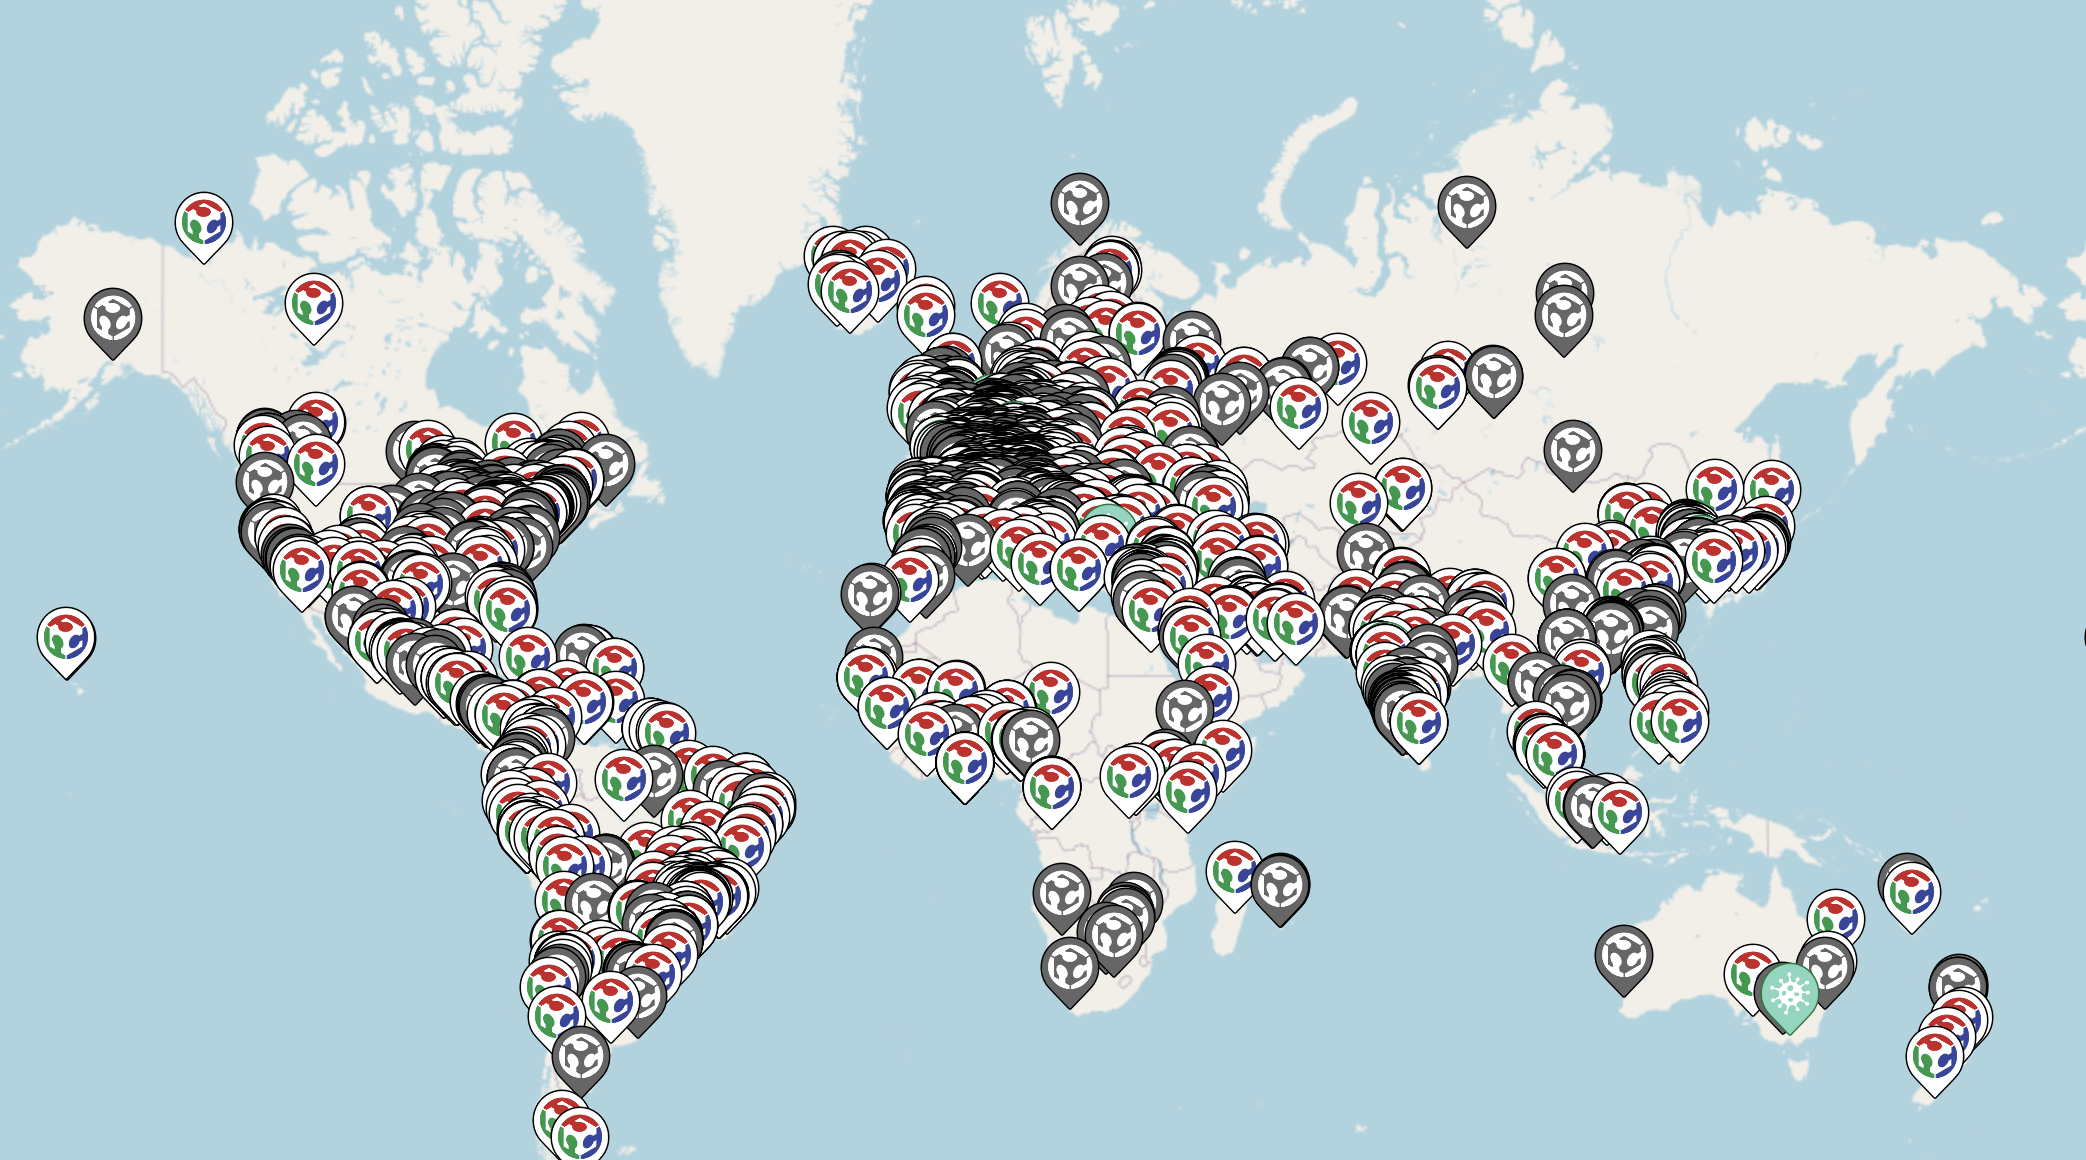
\includegraphics[width=1\textwidth]{figures/chapter2/fablabsmap.png}
\caption{Global distribution of FabLabs showing the rapid expansion of access-based democratization. Source: Fab Foundation, 2024}
\label{fig:fablabs_map}
\end{figure}

This democratization of digital fabrication extends beyond physical tools to software infrastructures. Open-source and free CAD alternatives like FreeCAD, Blender or TinkerCAD combined with educational programs to know how to use the tools, have reduced barriers to digital design literacy. Contemporary maker spaces enable individual access to CNC machines, 3D printers, and laser cutters for modest fees (sometimes even for free), genuinely transforming the economic conditions of making.

\vspace{0.5cm}

\vspace{0.5cm}

\vspace{0.5cm}

\vspace{0.5cm}

\vspace{0.5cm}

\vspace{0.5cm}